\section{Finite Difference Discretization}

Finite difference methods (FDM) are simple and robust, and are widely used.
But they have their limitations, as we will see.
Here we consider exemplary the following finite difference.

\begin{theorem}[Finite Differences]
	Let \(h < 1\) and \(x \in \R\).
	For \(f: \R \to \R\) with \(f \in C^4\parentheses*{\brackets*{x - h, x + h}}\), the \emph{second order central difference}
	\[
		\delta_h^2\brackets*{f}\parentheses*{x} := \frac{f\parentheses*{x + h} - 2f\parentheses*{x} + f\parentheses*{x - h}}{h^2}
	\]
	satisfies \(f''\parentheses*{x} = \delta_h^2\brackets*{f}\parentheses*{x} + Ch^2\) for some \(C \le \frac{1}{12}\norm*{f^{\parentheses*{4}}}_\infty\).
\end{theorem}

\begin{proof}
	Taylor expansion see lecture ``Mathematische Grundlagen IV (CES)''.
\end{proof}

We now use the FDM with \(\delta_h^2\) to approximated the Poisson problem \(-\Delta u = f\) in the unit square \(\Omega = \brackets*{0, 1} \subset \R^2\) with Dirichlet boundary conditions \(u = g\) on \(\partial\Omega\).
We discretize by using the point-wise approximations \(u_{i, j} \approx u\parentheses*{x_i, y_j}\) on a uniform Cartesian grid
\[
	x_i = ih, y_j = jh, \quad i, j = 0, \ldots, N + 1, h = \frac{1}{N + 1}
\]
for \(N \in \N\).

\begin{figure}[h]
	\centering
	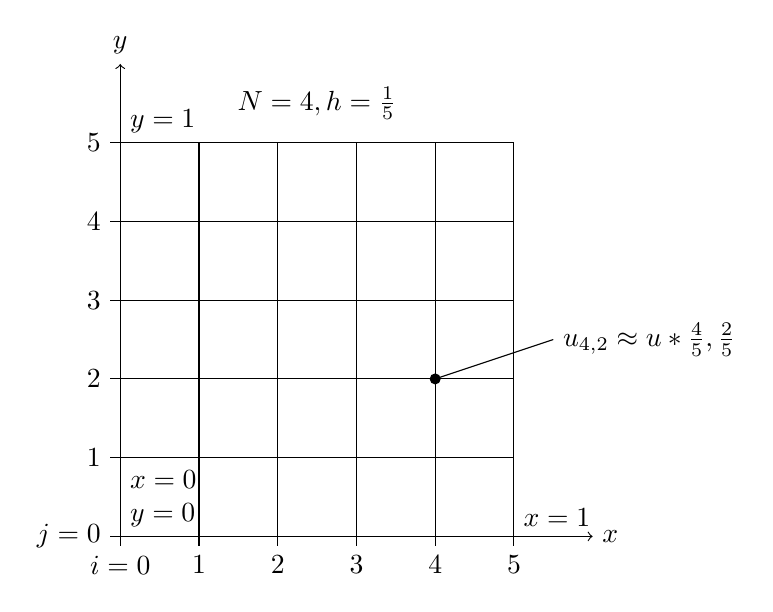
\begin{tikzpicture}
		\draw[<->] (0,6) node[above] {\(y\)} -- (0,0) -- (6,0) node[right] {\(x\)};
		\foreach \i in {1,...,5}
		{
			\draw (\i,.125) -- (\i,-.125) node[below] {\(\i\)};
			\draw (.125,\i) -- (-.125,\i) node[left] {\(\i\)};
			\draw (0,\i) -- (5,\i);
			\draw (\i,0) -- (\i,5);
		}
		\node at (2.5,5.5) {\(N = 4, h = \frac{1}{5}\)};
		\filldraw (4,2) circle (.0625);
		\draw (5.5,2.5) node[right] {\(u_{4, 2} \approx u\parentheses*{\frac{4}{5}, \frac{2}{5}}\)} -- (4,2);
		\draw (-.125,0) node[left] {\(j = 0\)} -- (0,0) -- (0,-.125) node[below] {\(i = 0\)};
		\node[anchor=south west,align=left] at (0,0) {\(x = 0\)\\\(y = 0\)};
		\node[anchor=south west] at (5,0) {\(x = 1\)};
		\node[anchor=south west] at (0,5) {\(y = 1\)};
	\end{tikzpicture}
	\caption{A uniform Cartesian grid with parameters \(N = 4\) and \(h = \frac{1}{5}\)}
	\label{fig:1-1}
\end{figure}

For every interior point \(\parentheses*{x, y} \in \braces*{\parentheses*{x_i, y_j} : 1 \le i, j \le N}\) we thus have
\begin{align*}
	-\partial_{xx}u\parentheses*{x, y} - \partial_{yy}u\parentheses*{x, y} &= f\parentheses*{x, y}, && \text{(continuous equation)},\\
	-\frac{u\parentheses*{x + h, y} - 2u\parentheses*{x, y} + u\parentheses*{x - h, y}}{h^2} - \frac{u\parentheses*{x, y + h} - 2u\parentheses*{x, y} + u\parentheses*{x, y - h}}{h^2} &= f\parentheses*{x, y}, && \text{(finite differences)}.
\end{align*}


\subsection{Stencil and Discretization}

For a system of equations for \(u_{i, j}\) we set \(x = x_i\) and \(y = y_i\) for
\[
	-\frac{u_{i + 1, j} - 2u_{i, j} + u_{i - 1, j}}{h^2} - \frac{u_{i, j + 1} - 2u_{i, j} + u_{i, j - 1}}{h^2} = f_{i, j}, \quad i, j = 1, \ldots, N
\]
which gives the so-called \emph{\(5\)-point-stencil} as shown in Figure \ref{fig:1-1}.

\begin{figure}[h]
	\centering
	\begin{tikzpicture}
		\foreach \p in {(0,0),(-2,0),(0,2),(2,0),(0,-2)}
		{
			\filldraw \p circle (.0625);
			\draw \p -- (0,0);
		}
		\node[anchor=north west] at (0,0) {\(\parentheses*{i, j}\)};
		\node[anchor=south east] at (0,0) {\(-4\)};
		\node[anchor=north] at (-2,0) {\(\parentheses*{i - 1, j}\)};
		\node[anchor=south] at (-2,0) {\(1\)};
		\node[anchor=east] at (0,2) {\(\parentheses*{i, j + 1}\)};
		\node[anchor=west] at (0,2) {\(1\)};
		\node[anchor=north] at (2,0) {\(\parentheses*{i + 1, j}\)};
		\node[anchor=south] at (2,0) {\(1\)};
		\node[anchor=east] at (0,-2) {\(\parentheses*{i, j - 1}\)};
		\node[anchor=west] at (0,-2) {\(1\)};
	\end{tikzpicture}
	\caption{A visual representation of the \(5\)-point-stencil}
	\label{fig:1-1}
\end{figure}

The boundary terms \(u_{0, j}, u_{N + 1, j}\) and \(u_{i, 0}, u_{i, N + 1}\) for \(i, j = 1, \ldots, N\) can be replaced by the boundary conditions \(u = g\), that is, by the values \(g_{0, j}, g_{N + 1, j}\) and \(g_{i, 0}, g_{i, N + 1}\).
The unknown values \(u_{i, j}\) with \(i, j = 1, \ldots, N\) are sorted into a large single vector
\[
	U_h = \parentheses*{u_{1, 1} \ldots, u_{N, 1}, u_{1, 2}, \ldots, u_{N, N}}^T \in \R^{N^2}.
\]
This yields a linear system of equations
\[
	-A_h U_h = F + G, \quad F = \begin{pmatrix}
		f_{1, 1}\\
		\vdots\\
		f_{N, 1}\\
		f_{1, 2}\\
		\vdots\\
		f_{N, N}
	\end{pmatrix}, \quad G = \frac{1}{h^2}\begin{pmatrix}
		g_{1, 0} + g_{0, 1}\\
		g_{2, 0}\\
		\vdots\\
		g_{N, 0} + g_{N + 1, 1}\\
		g_{0, 2}\\
		\vdots\\
		g_{N, N + 1} + g_{N + 1, N}
	\end{pmatrix}
\]
with \(F, G \in \R^{N^2}\) and
\[
	A_h = \frac{1}{h^2}\begin{pmatrix}
		T & -I & 0 & \cdots & 0\\
		-I & T & \ddots & \ddots & \vdots\\
		0 & \ddots & \ddots & \ddots & 0\\
		\vdots & \ddots & \ddots & T & -I\\
		0 & \cdots & 0 & -I & T
	\end{pmatrix}, \quad T = \begin{pmatrix}
		4 & -1 & 0 & \cdots & 0\\
		-1 & 4 & \ddots & \ddots & \vdots\\
		0 & \ddots & \ddots & \ddots & 0\\
		\vdots & \ddots & \ddots & 4 & -1\\
		0 & \cdots & 0 & -1 & 4
	\end{pmatrix}
\]
with identity matrix \(i \in \R^{N \times N}\).

\begin{remark}
	\begin{enumerate}
		\item Remarkably, the PDE has been reduced to a linear algebraic system.
		\item \(A_h\) is symmetric, positive definite and sparse, that is, it contains many zeros, this allows to use efficient linear solvers.
		\item Both the source term and boundary conditions enter the system as inhomogenities on the right-hand side.
	\end{enumerate}
\end{remark}


\subsection{Quality of the Approximation}


Let's denote the interior point values of the exact solution of the Poisson problem as
\[
	U_{\text{ex}} = \parentheses*{u\parentheses*{x_1, y_1}, u\parentheses*{x_2, y_1}, \ldots, u\parentheses*{x_N, y_N}}^T.
\]
We are interested in the error \(\norm*{U_h - U_{\text{ex}}}\) in a norm of our choice.

\begin{definition}
	A FDM with the lineare system \(A_h U_h = Q\) is called
	\begin{enumerate}
		\item \emph{consistent} of order \(p > 0\) if \(\norm*{A_h U_{\text{ex}} - Q} \le C_1 h^p\),
		\item \emph{stable} if \(\norm*{A_h^{-1}} \le C_2\),
	\end{enumerate}
	for all \(h > 0\) sufficiently small.
\end{definition}

Notice that the stability defintion can equivalently be stated as \(\norm*{A_h V} \ge C_2^{-1}\norm*{V}\) for all \(V \not\in \ker\parentheses*{A_h}\).
Moreover, cosistency and stability guarantee convergence.

\begin{theorem}
	A stable FDM that is consistent of order \(p\) is also convergent with order \(p\), so that
	\[
		\norm*{U_h - U_{\text{ex}}} \le Ch^p.
	\]
\end{theorem}

\begin{proof}
	A direct computation gives
	\begin{align*}
		\norm*{U_h - U_{\text{ex}}} &= \norm*{A_h^{-1}A_h\parentheses*{U_h - U_{\text{ex}}}}\\
		&= \norm*{A_h^{-1}\parentheses*{A_h U_h - A_h U_{\text{ex}}}}\\
		&\le \norm*{A_h^{-1}}\norm*{Q - A_h U_{\text{ex}}}\\
		&\le C_2 C_1 h^p.
	\end{align*}
\end{proof}

Applied to our running example for the Poisson problem discretized by the second order central difference on the unit square eventually yields the following.

\begin{theorem}
	The above FDM discretization for the Poisson problem based on the \(5\)-point-stencil is second order convergent and satisfies
	\[
		\norm*{U_h - U_{\text{ex}}}_\infty \le \frac{h^2}{192}\parentheses*{\norm*{\partial^{\parentheses*{4, 0}}u_{\text{ex}}}_\infty + \norm*{\partial^{\parentheses*{0, 4}}u_{\text{ex}}}_\infty},
	\]
	provided that the exact solution is \(u_{\text{ex}} \in C^4\parentheses*{\Omega}\).
\end{theorem}

\begin{proof}
	Exercise.
\end{proof}


\subsection{Limitations and criticism of FDMs}

\begin{enumerate}
	\item\label{enum:1-1} The extension to non-Cartesian domains is difficult, because points close to the boundary require special finite differences.
	\item\label{enum:1-2} Different tyles of boundary conditions, e.g. Neumann conditions, are not straight-forward to incorporate.
	For example, the condition \(n\grad u = g_N\) would need to be discretized with appropriate, special finite differences and would require an equation for the boundary values of \(u_{i, j}\).
	\item Higher order of consistency \(\mathcal{O}\parentheses*{h^p}\) with \(p > 2\) requires a larger stencil width, so that \(A_h\) becomes denser.
	This implies even more problems close to the boundary; see \ref{enum:1-1} and \ref{enum:1-2}.
	\item The convergence theory requires very strong conditions on the regularity (i.e. smoothness) of the exact solution.
	For example, even for the simple Poisson problems on \(\brackets*{0, 1}^2\) we require \(u_{\text{ex}} \in C^4\), that is, four continuous derivatives.
\end{enumerate}


\subsection{Non-Smooth Boundaries}

What regularity (i.e. how many continuous derivatives) can we expect from the solution of \(-\Delta u = f\)?

\begin{theorem}[Smooth Poisson]
	If \(\Omega\) has a smooth boundary (no corners), in the sense that \(\partial\Omega\) can be parameterized in \(C^\infty\), then the solution \(u\) of the Poisson problem satisfies
	\[
		f \in C^k\parentheses*{\Omega} \implies u \in C^{k + 2}\parentheses*{\Omega}.
	\]
\end{theorem}

\begin{example}[Pacman-Poisson]
	Consider the Poisson problem on the ``Pacman''-domain \(\Omega_\alpha\), which is opened by an angle \(\alpha \in \parentheses*{0, 2\pi}\).
	Using polar coordinates, the domain thus is
	\[
		\Omega_\alpha = \braces*{\parentheses*{x, y} = r\parentheses*{\cos\varphi, \sin\varphi} : r \in \parentheses*{0, R}, \varphi \in \parentheses*{0, \alpha}}
	\]
	and the problem statement reads
	\[
		\Delta u = 0, \quad \text{in }\Omega,
	\]
	with Dirichlet boundary conditions
	\[
		u = \begin{cases}
			\sin\parentheses*{\frac{\pi}{\alpha}\varphi}, & \text{on }\Gamma_1,\\
			0, & \text{on }\Gamma_0,
		\end{cases}
	\]
	so that the solution in polar coordinates is
	\[
		u\parentheses*{r, \varphi} = \parentheses*{\frac{r}{R}}^{\frac{\pi}{\alpha}}\sin\parentheses*{\frac{\pi}{\alpha}\varphi}.
	\]
	The derivative with respect to \(r\) satisfies
	\[
		\partial_r u\parentheses*{r, \varphi} = \frac{\pi}{\alpha}\frac{1}{R}\parentheses*{\frac{r}{R}}^{\frac{\pi}{\alpha} - 1}\sin\parentheses*{\frac{\pi}{\alpha}\varphi} \xrightarrow{r \to 0} \infty, \quad \text{if }\frac{\pi}{\alpha} - 1 < 0,
	\]
	which means that the solution has a singularity at the origin in its first derivative for \(\alpha > \pi\) (reentrant corner).
	That is, \(u \not\in C^1\parentheses*{\Omega}\).
	Similarly, we also find for the second derivative \(u \not\in C^2\parentheses*{\Omega}\), if \(\alpha > \frac{\pi}{2}\), and \(u \not\in C^3\parentheses*{\Omega}\), if \(\alpha > \frac{\pi}{3}\), etc.
\end{example}

\begin{remark}
	\begin{enumerate}
		\item As soon as \(\Omega\) has corners, the solution of the Poisson problem looses smoothnes.
		If the corner is reentrant, the solution at that corner is not even differentiable.
		\item This implies that we cannot expect ``nice'' convergence of the finite difference method.
		However, it may still work, for instance, if the stencil does not include the corners.
	\end{enumerate}
\end{remark}
